\documentclass[12pt]{article}
\input{/Users/circle/Documents/博一上/homework/setting.tex}
\setcounter{secnumdepth}{2}
\usepackage{bm}
\usepackage{autobreak}
\usepackage{amsmath}
\graphicspath{{../}}
\setlength{\parindent}{2em}
\newcommand{\bs}  [1]{\boldsymbol{#1}}

%pdf文件设置
\hypersetup{
	pdfauthor={袁磊祺},
	pdftitle={Advanced Fluid Mechanics Homework 5}
}

\title{
		\vspace{-1in} 	
		\usefont{OT1}{bch}{b}{n}
		\normalfont \normalsize \textsc{\LARGE Peking University}\\[1cm] % Name of your university/college \\ [25pt]
		\horrule{0.5pt} \\[0.5cm]
		\huge \bfseries{Advanced Fluid Mechanics Homework 5} \\
		\horrule{2pt} \\[0.5cm]
}
\author{
		\normalfont 								\normalsize
		College of Engineering \quad 2001111690  \quad 袁磊祺\\	\normalsize
        \today
}
\date{}

\begin{document}

\input{setc.tex}

\maketitle

\section{1}

\begin{equation}
	\frac{u}{U}=1-\exp \left(-\frac{v_{0} y}{\nu}\right)
\end{equation}
边界层位移厚度
\begin{equation}
	\delta^* = \int^{\infty}_0 \frac{U-u}{U} \dif y = \int^{\infty}_0 \exp \left(-\frac{v_{0} y}{\nu}\right) \dif y = \frac{\nu}{v_{0}}.
\end{equation}
粘性系数
\begin{equation}
	\mu = \nu \rho,
\end{equation}
表面摩擦力
\begin{equation}
	\tau_0 = \mu  \frac{\dif u}{\dif y}\Big|_{y=0} = \rho U v_0.
\end{equation}



\section{2}

先统一一下符号标记
\begin{gather}
	x = z,\\
	\sigma = r,\\
	v = u_\theta.
\end{gather}

由\emph{Vortical Flows}中的(6.1.8b), 对于无粘情况, 
\begin{equation}
	\frac{\Dif}{\Dif t}\left(\frac{\omega_{\theta}}{r}\right)=\frac{1}{r^{4}} \frac{\partial C^{2}}{\partial z}=\frac{2C}{r^{4}} \frac{\partial C}{\partial z},
\end{equation}
其中
\begin{equation}
	C = vr.
\end{equation}
又根据(6.1.4a)
\begin{equation}
	\omega_r = - \frac{1}{r} \frac{\partial C}{\partial z},
\end{equation}
\begin{equation}
	\frac{\Dif}{\Dif t}\left(\frac{\omega_{\theta}}{r}\right)=  -\frac{2v\omega_r}{r^2}.
\end{equation}\qed

\section{3}

在轴对称假设下, 流体的动能为
\begin{equation}
	T = \pi \rho \int^{+\infty}_{-\infty} \int^{+\infty}_{0} \left(\psi \omega_\theta + V^2_\theta r \right)\dif r \dif z.
\end{equation}
对于Hill球涡, 
\begin{gather}
	V_\theta = 0,\\
	\omega_\theta (r,z)= \begin{cases}
		-\frac{15}{2}\frac{U}{a^2}r, &R = \sqrt{r^2+z^2}<a,\\
		0, &R = \sqrt{r^2+z^2}>a,
	\end{cases}
\end{gather}
\begin{gather}
	\psi (r,z)= \begin{cases}
		-\frac{3}{4}Ur^2\left(1-\frac{R^2}{a^2}\right)-\frac{3}{4}Ur^2\left(1-\frac{R^2}{a^2}\right)-\frac{1}{2}Ur^2, &R = \sqrt{r^2+z^2}<a,\\
		\frac{1}{2}Ur^2\left(1-\frac{a^3}{R^3}\right) -\frac{3}{4}Ur^2\left(1-\frac{R^2}{a^2}\right)-\frac{1}{2}Ur^2, &R = \sqrt{r^2+z^2}>a.
	\end{cases}
\end{gather}
积分可得
\begin{equation}
	T = \pi \rho \int^{a}_{-a} \int^{+\sqrt{a^2-z^2}}_{0} \left(\psi \omega_\theta \right)\dif r \dif z = \frac{10}{7}\pi \rho U^2 a^3.
\end{equation}

\section{4}

在极坐标下, 方程
\begin{equation}
	\nabla^{2} \psi=c \psi
\end{equation}
写为
\begin{equation}
	\frac{1}{r} \pd{}{r}\left(r\frac{\partial \psi}{\partial r}\right) + \frac{1}{r^2} \pd[2]{\psi}{\theta} = c\psi.
	\label{eq:41}
\end{equation}
把式子
\begin{equation}
	\psi^{(i)}=c J_{1}(k r) \sin \theta
	\label{eq:42}
\end{equation}
代入\cref{eq:41} ,并假设$c<0,\ \sin \theta \not=0,\ x=kr$可得
\begin{equation}
	x^2 J_1'' + xJ_1'-\left(\frac{c}{k^2}x^2 + 1 \right)J_1=0.
\end{equation}
当$k=\sqrt{-c}$时, \cref{eq:42}正好是$m=1$的贝塞尔方程的解. 

在极坐标下, 流函数和速度的关系为
\begin{equation}
	v^{(i)}_\theta = -\pd{\psi^{(i)}}{r}= - ck J'_{1}(k r) \sin \theta,\quad v^{(i)}_r = \frac{1}{r} \pd{\psi^{(i)}}{\theta}=  \frac{c}{r}  J_{1}(k r) \cos \theta.
\end{equation}
$v_r=0$时
\begin{equation}
	J_1(kr_0) = 0.
\end{equation}
假设$kr_0$是$J_1$的第一个零点, 则
\begin{equation}
	v^{(i)}_\theta = - ck J'_{1}(k r_0) \sin \theta.
\end{equation}

均匀来流的流函数
\begin{equation}
	\psi^{(o)} = U_{\infty}\left(1-\frac{a^{2}}{r^{2}}\right) r \sin \theta, \quad a = r_0.
\end{equation}
速度
\begin{equation}
	v^{(o)}_\theta = - \pd{\psi^{(o)}}{r}= - U_{\infty}\left(1+\frac{a^{2}}{r^{2}}\right) \sin \theta, \quad v^{(o)}_r = \frac{1}{r} \pd{\psi^{(o)}}{\theta}= U_{\infty}\left(1-\frac{a^{2}}{r^{2}}\right)  \cos \theta.
\end{equation}
匹配
\begin{equation}
	v^{(o)}_\theta (r=a) = v^{(i)}_\theta (r=a)
\end{equation}
得
\begin{equation}
	U_{\infty} = ck J'_{1}(k r_0)/2.
\end{equation}
得内外流函数
\begin{equation}
	\psi = 
	\begin{cases}
		c J_{1}(k r) \sin \theta, & r<a,\\
		\frac{1}{2}ck J'_{1}(k r_0)\left(1-\frac{a^{2}}{r^{2}}\right) r \sin \theta, & r>a.
	\end{cases}
\end{equation}
其中$k=\sqrt{-c},\ a=r_0$.

假设$c=-1$, 对于一阶贝塞尔函数, $r_0 = 3.8317$, 去流函数等值面, 可得流线图, 如\cref{fig:4} 所示. 

\begin{figure}[htp]
	\centering
	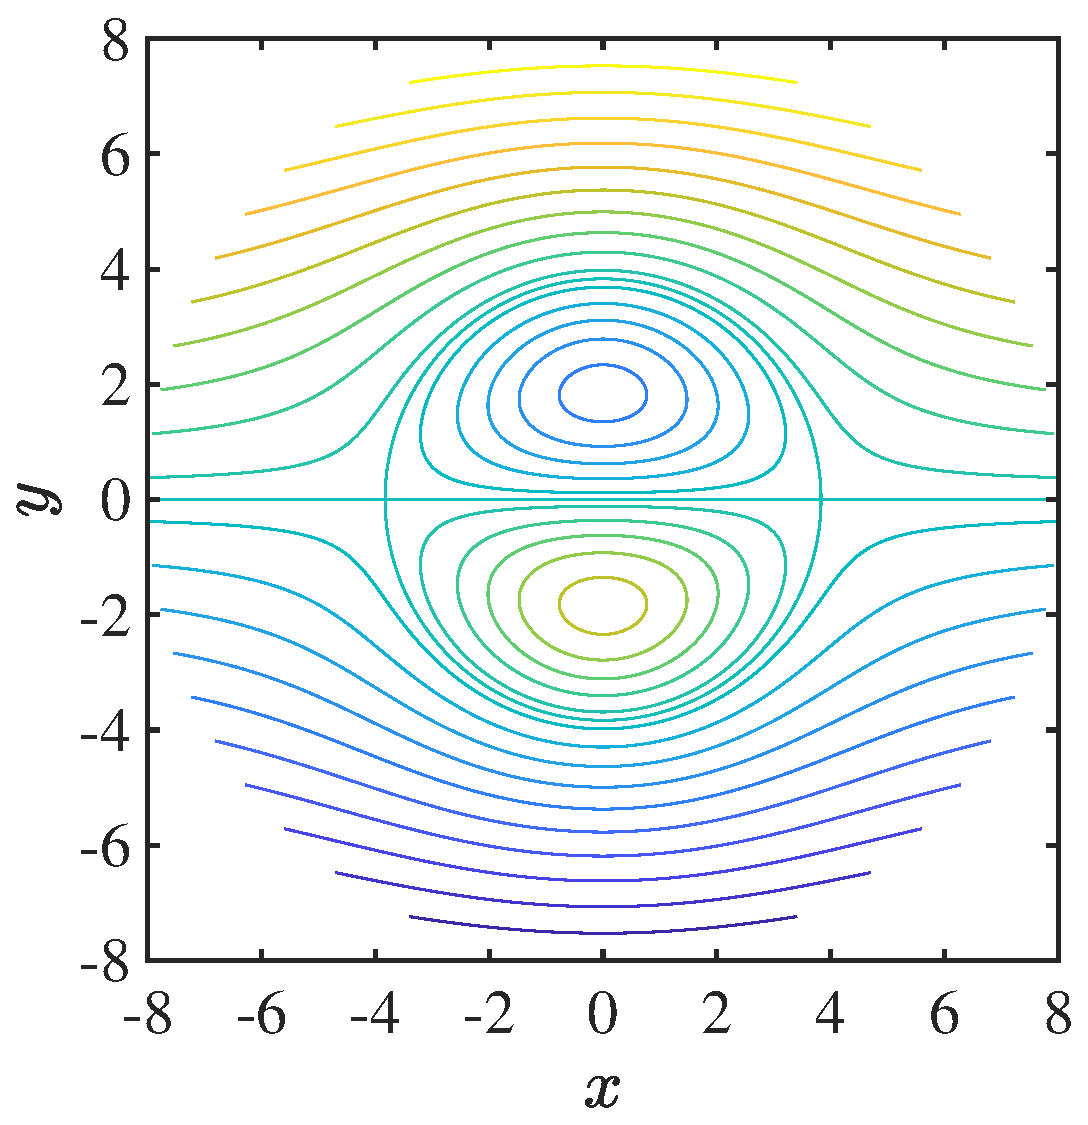
\includegraphics[width=7cm]{4.eps}
	\caption{流线图.}
	\label{fig:4}
\end{figure}


\section{5}

如\cref{fig:5} 所示, 从右上角顺时针绕一圈, 箭头先从东北方向向北旋转, 然后返回为东北方向, 然后再重复一遍, 所以该奇点的指标为0. 

\begin{figure}[htp]
	\centering
	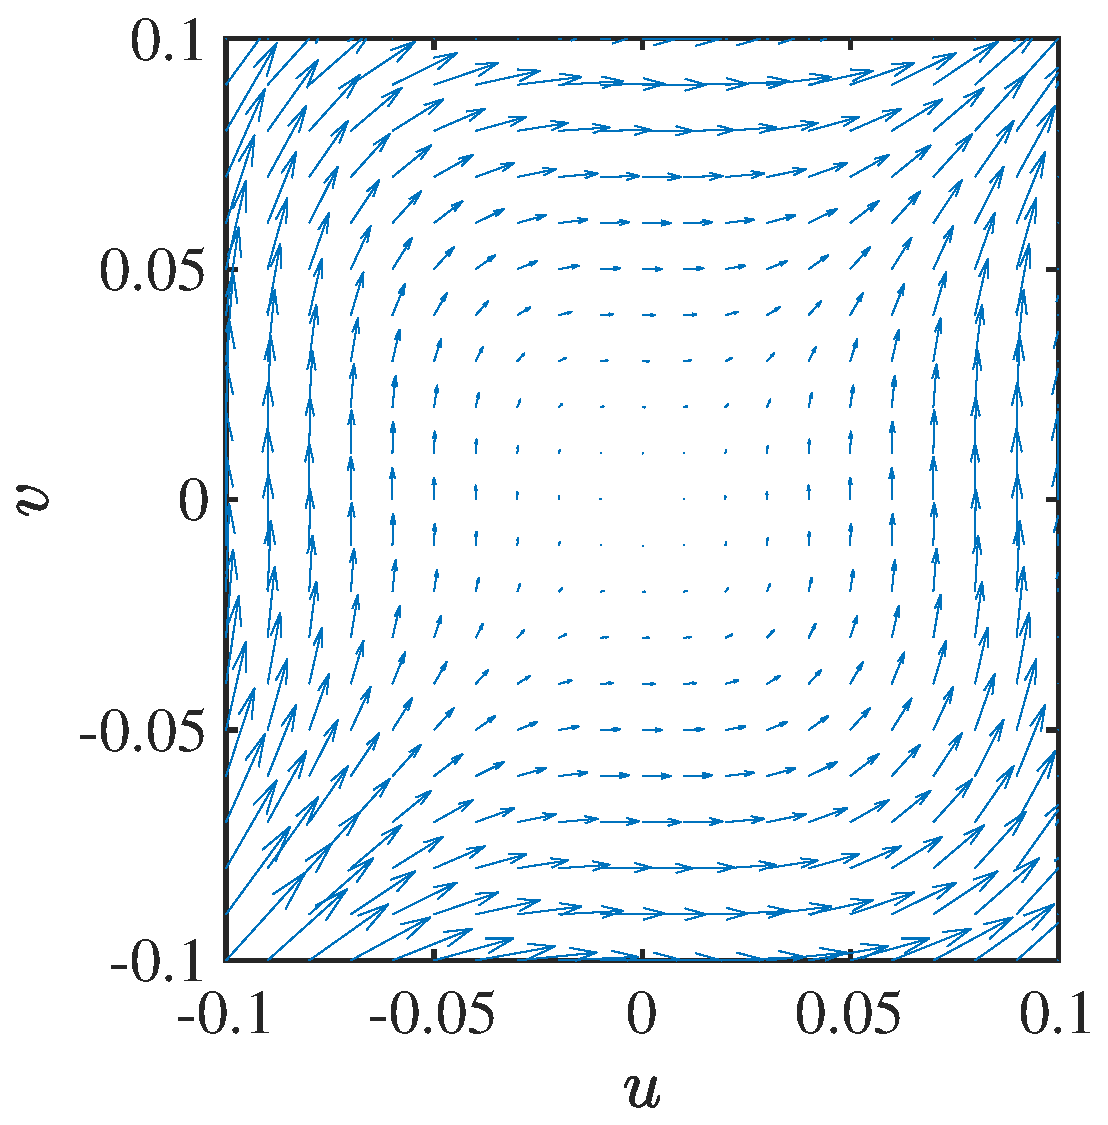
\includegraphics[width=7cm]{5.eps}
	\caption{流场矢量图.}
	\label{fig:5}
\end{figure}

\section{6}

由于 $\left(\frac{\partial^{2} w}{\partial z^{2}}\right)_{0}=-\left[\frac{1}{h_{1}}\left(\frac{\partial^{2} u}{\partial x \partial z}\right)+\frac{1}{h_{2}}\left(\frac{\partial^{2} v}{\partial y \partial z}\right)\right]_{0}$, 判定流动分离的条件是:在分离线上
\begin{equation}
	\begin{cases}
		\left(\frac{\partial u}{\partial z}\right)_{0}=0, \\
		\left(\frac{\partial^{2} u}{\partial x \partial z}\right)_{0}<0, \\
		\left(\frac{\partial^{2} w}{\partial z^{2}}\right)_{0}>0 \text { 或 }\left(\frac{1}{h_{1}} \frac{\partial^{2} u}{\partial x \partial z}+\frac{1}{h_{2}} \frac{\partial^{2} v}{\partial y \partial z}\right)_{0}<0.
	\end{cases}
\end{equation}
对应于书上的
\begin{align}
	\tau_{x, x} &>0, \\
	\tau_{y} &=0, \quad \tau_{y, x}=0, \\
	\tau_{y, y} &<0, \\
	\nabla_{\pi} \cdot \boldsymbol{\tau} &=\tau_{x, x}+\tau_{y, y}<0.
\end{align}
注意两书的$x,y$标号是反的. 

我从图书馆借了书, 书内容太多, 之前的部分我就不抄了. 



\section{7}

根据三角翼的升力公式
\begin{equation}
	L \approx \rho U \int_W y \omega_x \dif S,
\end{equation}
由于三角翼会卷起一个很强的涡, 并且是延着$x$方向, 即$\omega_x$很大, 所以升力也很大. 

如\cref{fig:7} 所示, 发动机的转子布满一圈三角形的叶片, 图示是正视图, 转动方向如图中箭头所示. 

\begin{figure}[htp]
	\centering
	\includegraphics[width=7cm]{7.jpeg}
	\caption{发动机转子示意图.}
	\label{fig:7}
\end{figure}



\nocite{*}

\input{bib.tex}

\end{document}
